\documentclass[english,dit,report]{hogentreport}

\usepackage{lipsum}
\usepackage{subcaption}

\graphicspath{{img/}}

\addbibresource{examples.bib}  % Voorbeelden voor het hst over bibliografie
\addbibresource{references.bib}  % Referenties in de tekst

\author{Thomas Aelbrecht, Lena {De Mol}, Koen Mertens, Bert {Van Vreckem}}
\title[IT Syllabus]{Research Methods}
\academicyear{2021--2022}

\begin{document}

\maketitle

\chapter*{Preface}
\label{ch:preface}

This guide orginated from the guidance process of the bachelor theses in the applied computer sciences department of HOGent and was originally published in Dutch via  Github\footnote{\url{https://github.com/HoGentTIN/bachproef-gids/}}. The idea was to give the students useful advice regarding methodology and working with {\LaTeX} for a professional layout, but also, to get them started on time.

In the new curriculum, that was introduced from the academic year 2020--2021, a new course i.e. ``Research methods'' was introduced mainly to support the bachelor thesis writing process. This bachelor thesis guide is then further developed and used as the course text for the new subject.

The objective of the bachelor thesis within the study program is to demonstrate that you are able to serve a ``customer'' (within their own organization or externally) \textbf{with advice about the application of current ICT technology in a business context. } We are not aiming for an academic scientific study, but we target applied research with sufficient technical depth offering added value in the chosen field.

This means that you get to work with a concrete and current problem from the field. You may not be an expert on this topic (yet), forcing you to gather relevant, objective, and authoritative information on that topic. On the one hand, this involves looking up existing knowledge that can be found in the professional literature, via experts or stakeholders. On the other hand, we expect that new knowledge will also be created during the research, for example through self-designed experiments, a proof-of-concept or prototype, interviews, etc. All this information should then be structured and analysed. In the case of quantitative data this should happen in a statistically sound way. Based on this, you can work out a solution and formulate your advice for the customer or client. You compile all this information in a thesis that you submit and defend before a jury.

Hopefully this course offers sufficient guidance to successfully start working on your bachelor's thesis!

\bigskip
Revision: \today

%---------- Inhoudstafel ------------------------------------------------------
%\usechapterimagefalse

\tableofcontents % Print the table of contents itself

%\cleardoublepage % Forces the first chapter to start on an odd page so it's on the right

%---------- Corpus ------------------------------------------------------------

\chapter*{Study Guide}
\label{ch:studyguide}
\addcontentsline{toc}{chapter}{Study Guide}

\section{Target and positioning of the course in the curriculum}
\label{sec:targetandplace}

The target of this course is to prepare the student for writing a bachelor thesis. More specifically, we want to support students with:

\begin{itemize}
  \item Searching for and formulating a research question;
  \item Searching for information in professional literature (literature study);
  \item The setup of a bibliographic database and the correct referencing of sources; 
  \item Applying appropriate research methods;
  \item Making use of the {\LaTeX} typesetting system for a professional layout;
  \item Clear and correct communication about research
\end{itemize}

There is no previous knowledge required to follow the course. A credit for the subject is a formal prerequisite for writing the bachelor thesis. 

\section{Study targets and competences}
\label{sec:studytargets}

Please check the study details on the Chamilo platform.

\begin{itemize}
  \item Formulating a research question
        \begin{itemize}           
          \item The student is able to explain the characteristics of a good research question
          \item The student is able to formulate a research question and defend why it is a good research question
          \item The student can split a research question into specific sub-questions and related objectives
          \item The student is able to explain and distinguish the different types of research
          \item The student is able to explain the different research methods and distinguish their suitability for a specific problem
        \end{itemize}

  \item Literature study
        \begin{itemize}               
          \item The student is able to explain the criteria of qualitative professional literature
          \item The student can distinguish between different types of sources
          \item The student can adjust his/her search strategy in function of the search results
          \item The student can consult professional literature in relation to a theme
          \item The student can extract the main concepts from professional literature
          \item The student can explain characteristics of a structured text
          \item The student can write a structured text
          \item The student can explain the importance of correct referencing
          \item The student can reference literature correctly
        \end{itemize}

  \item Research methods
        \begin{itemize}                  
          \item The student can select a research method in function of the problem at hand
          \item The student is able to carry out a research method in function of the problem 
          \item The student is able to distinguish between methods to collect quantitative data and is able to apply them correctly
          \item The student is able to distinguish between qualitative data collection methods 
        \end{itemize}

  \item Reporting
        \begin{itemize}        
           \item The student is able to format a document in a correctly structured manner and provide references by means of text typesetting software.
        \end{itemize}
\end{itemize}

\section{Content}
\label{sec:studycontent}
This course is subdivided into two major parts. In the IT part, the focus is on the technical part, e.g. searching for a suitable subject, looking up information in professional literature, etc. The language part offers support in clear communication: analyzing texts, adopting a professional writing style, avoiding typical language errors, etc. .

In this document you will mainly find the content of the IT part.

Module~\ref{ch:preparation} helps to set up a working environment, in particular the text typesetting system {\LaTeX} and a version control system.

Module~\ref{ch:researchquestion} provides tips on topic choice and how to work out a topic.

Module~\ref{ch:literaturestudy} provides details on how to perform a literature study. The subsequent module~\ref{ch:bibliography} teaches how to keep references centralized in a bibliographic database facilitating the insertion of a correct bibliography in a {\LaTeX} document.

Module~\ref{ch:researchmethods} elaborates on a set of research methods typically used in a bachelor thesis, i.e. \ the comparison between different methods, or the setup of experiments. 

Finally, module~\ref{ch:reportingresults} provides information regarding the more technical aspects of writing a thesis, and some {\LaTeX} specific guidelines.

\section{Study material}
\label{sec:studymaterial}

All the learning material for this course is provided to the students using the Chamilo platform. 

\section{Teaching approaches}
\label{sec:teachingapproach}

In this course, 12 contact moments of two hours are budgetted, alternating between IT and language classes. The order may vary depending on the student group. In the table below you will find more details on the content of the course in the different classes. 

An overview is provided in Table~\ref{tab:planning}.

\begin{table}
  \centering\begin{tabular}{cll}
    \toprule
    \textbf{Module} & \textbf{IT part}               & \textbf{Language part}                   \\
    \midrule
    1               & Preparation, {\LaTeX}        & Professional text structure \\
    2               & Formulating a research question & Professional writing     \\
    3               & Literature study               & Common language mistakes                 \\
    4               & Referencing correctly              & Evaluating sources   \\
    5               & Research methods             & Writing a summary          \\
    6               & Reporting                    & Presentation skills       \\
  \end{tabular}
  \caption{\label{tab:planning}Course content for the different classes of this course.}
\end{table}

\section{Work and study guidelines}
\label{sec:workstudyguidelines}

TODO

\section{Study counselling and planning}
\label{sec:studycounsellingplanning}

TODO

\section{Evaluation}
\label{sec:evaluation}
The evaluation for this course is based on a paper, written by each student individually or in groups of 2 students. In this paper you will develop a topic that may be suitable for writing a bachelor's thesis. You formulate an appropriate research question, conduct an initial literature study on the research domain and describe your research approach.

There is however no strict requirement that you should pick this subject for your bachelor's thesis. Hopefully you will gain expert knowledge and maturity in the specialization courses yet to be followed, possibly providing some extra inspiration. However, by performing the exercise within this course, you will have a better idea of what to expect from the bachelor's thesis. The process is supposed to train some necessary skills needed to write your bachelor's thesis. 

The result is assessed by both the IT lecturer and the language lecturer, each focussing on their expertise. E.g. the IT lecturer pays attention to the quality of the referenced sources, correct use of {\LaTeX}, etc., while the language lecturer looks at the structure, writing style and correct language use.

The assessment criteria will be published on Chamilo in the form of a Rubrics evaluation card.
\chapter{Preparation, working with \LaTeX{}}
\label{ch:preparation}

In this chapter we treat the initial work, starting to write a bachelor's thesis. You will find some recommendations on useful tools and the research process.

\section{{\LaTeX} use}
\label{sec:latex-use}

Most students are used to writing formatted text in a classic word processor environment (typically MS Word). For your bachelor's thesis it is advisable to abandon this habit.

Word, especially with the default template, produces a layout that is not suitable for publication. Once the length and complexity of a Word document increases (and it certainly does with a thesis), you will have to deal with inconsistencies in the layout of your text, page numbering and poorly positioned images.

When you copy text from another (preparatory) document or from a website, the original layout is copied. If it's not consistent with your main document, you'll have to adjust everything. This is a very time consuming and error prone job.

A classic word processor based on the WYSIWYG principle\footnote{What You See Is What You Get}, allows you to fine-tune the positioning of the text in the paper, but actually this great freedom will turn out as a disadvantage in this case. A sleek and professional design is a specialty that requires great attention to often finicky details. As a computer scientist, we do not have the necessary knowledge to realize this. Moreover, when you spend a significant amount of time designing your document, you are distracted from the core goal: the content of the text!

Another disadvantage of the classic word processor is the binary file format. This makes it impossible to put a document into a version control system (see Section~\ref{sec:versioncontrolsystem}). Soon different versions of the document start to live side by side: `bach ​​test 3.docx', `bach ​​test 5 March 30.docx', `final draft.docx', `final draft after feedback.docx', `final final draft. docx' \dots. You have versions on your laptop, on dropbox, on your fixed PC and in your mailbox. In the long run, the overview is lost, you forget to copy pieces of text or you make other mistakes.

{\LaTeX} is recommended for formatting a long text with a professional and sleek design. As you know, this is a \emph{text typesetting system} with a markup language (like HTML) that specializes in formatting text on paper. You write source code in {\LaTeX} markup, a `compiler' generates a PDF. {\LaTeX} is text based, so you can put this in a version control system.

Admittedly, {\LaTeX} does have some drawbacks. There's a learning curve that shouldn't be underestimated, and as long as you stick to the habits you've picked up from working with a word processor, {\LaTeX} won't always do what you expect. But most effort is required in the beginning to master {\LaTeX}. When writing a bachelor's thesis with a word processor, you have most work at the end, to get rid of all the imperfections, inconsistencies and errors in the design. At that point, you usually don't have enough time for that anymore, because the deadline is approaching. The result is almost always a document that is insufficiently finished and looks very unprofessional to the reader. This is not appropriate for a paper that serves as the conclusion of a \textit{professional} bachelor's degree.

For the rest of this guide, we'll assume you're using {\LaTeX}. Yet, this is not intended to be a {\LaTeX} manual, there are plenty of other sources available for that~\parencite{Oetiker2015}.

You can find a {\LaTeX} template for preparing the bachelor's thesis in the Github repository \url{https://github.com/HoGentTIN/bachproef-latex-template}. Don't forget to change the language to English. You can download the template via the green button at the top right. Cloning the repository or creating a fork is not recommended. After all, doing this will provide you with the entire history of the template, which is not relevant to your work.


\section{Bibliographic database}
\label{sec:bibliografic-database}

A mandatory part of a bachelor's thesis is a literature study. This is to familiarize yourself with the research domain (see Chapter~\ref{ch:literaturestudy}). It is important to keep track of what you read, so that you can refer to your sources when writing the introduction. Referring to sources and setting up a bibliography must be done in a strictly defined manner. This is something that you don't have to do manually, there are several software packages that largely automate this: bibliographic databases.

A bibliographic database allows you to keep structured metadata about the works read: title, author, year, and such, but also (clickable) URLs, PDFs of articles, notes, etc.

There are several possibilities, but JabRef\footnote{\url{http://www.jabref.org/}} is perhaps the most interesting for our purposes. JabRef is an open source bibliographic database written in Java and ideally suited for working with {\LaTeX}. It uses the same file format as Bib{\LaTeX}, the bibliography system built into {\LaTeX}.

The way in which a bibliography and references in the text should be written is fixed. However, there are different formatting styles. One of these is the so-called \textbf{APA style} which comes from the American Psychological Association (APA). It is the main standard for publications in the field of social sciences. The official guide to the APA style is very extensive and can therefore be inconvenient to use. The {\LaTeX} template for the bachelor's thesis already has the APA style built-in, so you don't have to worry about the correct formatting at all. This happens automatically, provided you keep the bibliographic data (eg title, author, year of publication) correctly in Jabref. More about that in Section~\ref{sec:publicationsjabref}.

\textbf{Please note!!} The use of the APA style is mandatory throughout HOGENT. This applies to the layout of the bibliography as well as references to sources in the text.

\section{Version control system}
\label{sec:versioncontrolsystem}

Hopefully the advantages of a version control system do not need to be explained to a computer scientist? Always use a version control system like Git to keep track of your work. Also create a Github repository. This is a good backup system (provided you sync regularly with Github). It also allows you to easily share your work with your promoter. One of the properties of version control is that it is ideally designed to track changes in \emph{text files}. Binary file formats such as documents from a classic word processor are not suitable for this, which is an extra motivation for using \LaTeX{}.

The following things definitely belong in your repository:

\begin{itemize}
    \item \LaTeX{} source code of the bachelor's thesis.
    \item images to insert.
    \item source code of self-written scripts, benchmarks, experiments, proof-of-concepts, etc. This makes your experiments easier to reproduce and validate by third parties.
    \item raw experiment results (in text format, e.g. CSV), transcripts of interviews, etc.
    \item single notes, ideas, etc. Use Markdown for this and avoid Word-do\-cu\-ments.  
\end{itemize}

In short, \emph{all} artifacts resulting from your research belong in the repository. For work documents where you want formatted text, but where \LaTeX{} is overkill, use Markdown\footnote{\url{https://guides.github.com/features/mastering-markdown/}}.

What does \emph{not} belong in your repository:

\begin{itemize}
    \item Help files created when compiling \LaTeX{}. You can prevent these from being included in a repository by creating a \texttt{.gitignore} file\footnote{For example \url{https://github.com/github/gitignore/blob/master/TeX. gitignore}}. The \LaTeX{} template for the bachelor's thesis is already set up correctly.
    \item Large (binary) files such as ISOs, virtual machines (e.g.\ .ova), etc.
    \item PDFs of the articles/ebooks you have read (this is considered ``redistribution'' and is not allowed under copyright law).
    \item Binary files that change often, eg Word documents.
    \item Files automatically generated from code in Git, e.g. compiled code.    
\end{itemize}

A version control system only becomes really useful if you use it properly. So commit as often as possible, write clear commit messages and sync regularly with Github!

\section{Summary}
\label{sec:preparation-summary}

The key points of this chapter are:

\begin{itemize}
    \item To obtain a clean, professional layout, it is better to write your thesis in {\LaTeX} compared to a classic word processor;
    \item Use a \emph{reference manager} to maintain a bibliographic database (JabRef is recommended).
    \item Use a version control system to store all your work (Git is recommended);
\end{itemize}

\chapter{Formulating a research question}
\label{ch:researchquestion}

This chapter provides some suggestions on searching for a topic. The website of the HOGENT library also has some general advice about this\footnote{\url{https://bib.hogent.be/how-to/onderwerp-formuleren/inleiding/}}, this guide is specifically aimed at the bachelor applied Informatics.

We regularly receive offers from external parties on subjects that are suitable for a bachelor's thesis, but the offer is not large enough to provide all students with a subject. On the other hand, developing a subject yourself is an interesting opportunity to delve into a subject that you would like to continue with after graduation.

\section{Types of research}
\label{sec:researchtypes}

A bachelor's thesis does not have to try to imitate an academic master's thesis. The professional bachelor has its own value, so it is perfectly possible to excel within the specific uniqueness of this profile. The main difference lies mainly in the type of research that is conducted.

In \emph{fundamental research}, which is typically carried out at universities, the emphasis is on expanding our knowledge in general. For example, within computer science it can be about developing new and/or more efficient algorithms for problem solving. Whether the results of fundamental research are immediately applicable is of secondary importance.

\emph{Applied research}, on the other hand, tries to formulate an answer to a concrete question from the field. The researcher will then try to answer that question on the basis of the knowledge that is currently available (and published by subject matter experts). This may concern, for example, how a new technology can be applied concretely in a business context, making a choice between various alternative products or technologies, a preliminary research prior to developing an application, etc. In applied research, the target group is also very specific, for example a single company. We also notice that the topics introduced by companies are also the best developed and most often lead to a good bachelor's thesis.

\section{Research domain choice}
\label{sec:research}

The first step is to choose your research domain. This is something that no one can really help you with. Choose a domain that you are interested in, so that you can gain sufficient motivation to delve into it. Your chosen specialization in the final year may be a good starting point. What kind of job would you like to start after graduation? Which technologies, platforms, \ldots would you like to work with?

Search for current problems/challenges in your chosen field. It is important to take your time to ``immerse'' yourself in current events. This cannot be done overnight. It is more efficient to put some time into this regularly over a number of weeks (e.g.\ an hour every day). In the long run you should be able to recognize the most important themes that people are mainly working on at the moment and that could provide inspiration for your subject.

In Section~\ref{sec:searchingrelevantinformation} you will find some concrete tips and starting points on searching for relevant information. 

\section{Formulating research questions and targets}
\label{sec:formulatingresearchquestion}

Once you get a feel for recent changes on a topic, you typically also get to know the most important problems and points of discussion. These can lead to the formulation of your main research question, which you can further divide into more concrete sub-research questions.

A good research question for a bachelor's thesis starts from a real or at least realistic \textit{company case}, a concrete problem that a specific company struggles with. This immediately ensures a clear \textit{delimitation} of the subject. A research question that is too vague or general will never lead to a good bachelor's thesis.

For example, ``What is the best agile methodology for companies?'' is \textit{not} a good research question in that regard. There are several agile methodologies, and there's probably a good reason for that. There is no clear winner that is best suited for every business. If that were the case, then twenty years after the publication of the Agile Manifesto \autocite{BeckEtAl2001}, it would already be clear what the best methodology is. A suitable methodology depends on many factors: the company culture, the type of company, the type of IT solutions being developed, the size of the company, etc. If you formulate your research question too general, you will never be able to come to a conclusive conclusion. We have experienced this too often in the past. The student then writes in the conclusion ``The best solution depends on your preference and your specific situation.'' In other words, there is no conclusion. So start from a concrete case, e.g. company XYZ struggles with the delivery of software on time and within budget and wants to apply an agile methodology. What is the most appropriate methodology for their specific situation? This clearly defines the subject and its added value is immediately visible.

There is no conclusive answer to a good research question yet. Questions such as ``What is data mining?'', ``Which PHP frameworks are there?'', ``What is the history of the Cloud?'' are therefore not suitable, because the answer can be found quickly by search on Wikipedia or Google, or by checking relevant professional literature.

It is also important to immediately think about the expected result, the \textit{research objective}. Under what circumstances can you speak of a successful bachelor's thesis? What is the concrete end result that you want to achieve?

You can use the S.M.A.R.T. principle of \autocite{UchelenJungjohann2003} to formulate your research objective(s):

\begin{description}
    \item[Specific] Is the objective unambiguous? Is it clear who will benefit?
    \item[Measurable] Under which (measurable/observable) conditions or form has the goal been achieved? Is the goal to deliver a proof-of-concept or prototype? An analysis for an application to be developed? A comparison between possible alternative solutions with clear advice? etc.
    \item[Acceptable] Are these goals acceptable to the target audience? Will the target group actually be able to use the proposed solution?
    \item[Realistic] Is the goal achievable? Is the subject sufficiently defined? Is the difficulty of the problem at the professional bachelor level?
    \item[Time-bound] When (in time) should the goal be reached? This is clearly laid down for a bachelor's thesis: the deadline for submission. 
\end{description}

\section{Writing a research proposal}
\label{sec:researchproposal}

Once you have a research question, you can write out your topic to submit it for approval. This means that you will also be conducting some literature research. For instructions on how to approach this, see Chapter~\ref{ch:literature research}.

What you read about the subject, you have to structure and formulate in your own words in a continuous text. A good tool to organize your thoughts on a topic and to write a structured text around it later is to set up a mind map. There are various tools that you can use for free, such as XMind\footnote{\url{https://www.xmind.net/}} or FreeMind\footnote{\url{http://freemind.sourceforge.net/ }}.

% TODO: voorbeeld mindmap?

It is not the intention at this stage to write a fully detailed literature study, but a number of references are expected. After reading your proposal, your supervisor should understand the context of your research and why there is a problem that needs a solution. You must be able to demonstrate this on the basis of authoritative professional literature.

Also think about a title for your bachelor's thesis. It doesn't have to be final yet, but a good title makes it clear exactly which direction you want to go. A concrete title gives your supervisor(s) the confidence that you know exactly what you want to do and that this is a realistic goal. Try to keep the following in mind when formulating a title:

\begin{itemize}
    \item Do not formulate the title as a question.
    \item Avoid obscure jargon and do not use abbreviations. The title should also be understandable to someone outside your specific field.
    \item Just naming your professional domain is not enough because it is too vague. Your title should be specific and make it clear what exactly you want to research. That also means that a title can be long. For example, ``Cloud computing'' is a general term that covers a lot, and thus means nothing. ``The selection of an open source Infrastructure as a Service platform for setting up a test environment for web development'' is a lot more concrete.  
\end{itemize}

When assessing a subject, the following criteria are taken into account:

\begin{itemize}
 \item There is a concrete, \textbf{clearly defined research question}, research objective.
 \item The proposal is \textbf{innovative} and has a clear \textbf{added value} for a specific target group from the ICT field.
 \item The \textbf{methodology} is clearly justified, research techniques are suitable for answering research question
 \item There is a clear \textbf{personal contribution} and \textbf{technical draft}.
\end{itemize}

\section{Common mistakes}
\label{sec:subjectcommonmistakes}

The following things provide us with the idea that your subject has not yet been sufficiently worked out in depth or that there are still important common mistakes that stand in the way of a successful bachelor's thesis:

\begin{itemize}
  \item There is no concrete real or realistic \textbf{company case} associated with the topic. Research at bachelor level is applied, in other words we try to solve concrete, real problems. That should also be reflected in your subject.
  \item (One of) the research objective(s) is \textbf{speculation about the future} (e.g.  ``what will be the impact of the Internet of Things on everyday life?''). The conclusion of a bachelor's thesis must be verifiable, future predictions never are.
  \item The result of the research is \textbf{depending on external factors} to a large extent. For example, if you are going to conduct a survey, it is important to realize that it is not easy to find enough respondents. You will therefore immediately have to indicate how you intend to take a sufficiently large sample. Even if your plan is to conduct interviews with experts, companies, etc., it is important to make the necessary contacts before the start of your research. After all, if it is not possible to speak to the necessary people in time, the result of your bachelor's thesis will be in danger.
  \item The subject shows insufficient \textbf{technical depth}. The professional bachelor's degree in applied computer science is a technical profile and we expect you to demonstrate that you are technically strong. For example, a topic such as ``what is the most user-friendly mobile application for home banking for seniors?'' \textit{not} meets this requirement. These kinds of applications are developed by banks and as a student you will never have access to the internal workings. You may have to limit yourself to interviews and/or surveys with the target group. In this way you cannot demonstrate what you have to offer as a computer scientist.
  \item The \textbf{reference list} is too short or consists of unsuitable sources. Take the time to do an initial literature review and look beyond the first blog entry. In Chapter~\ref{ch:literature research} you will find instructions on how to approach this.
  \item The subject is \textbf{outside the scope of a bachelor's program or of the student}. Choose a subject that corresponds to a bachelor's degree in terms of level. A typical example of a subject that is too difficult is \textit{Quantum Computing}, at least for a bachelor's degree. Such a subject may be eye-catching, but with it you run the risk of shooting yourself in the foot in terms of difficulty.     
\end{itemize}

\section{Summary}
\label{sec:subjectsummary}

\begin{itemize}
 \item Take your time to find a topic that really interests you.
 \item When writing up a proposal, it is best to be as \emph{concrete} as possible.
 \item Avoid common mistakes such as the lack of a concrete case, speculation, dependence on external factors and a literature study that is too superficial.
\end{itemize}

\chapter{Literature study}
\label{ch:literaturestudy}

The first stage in any research is typically to write an overview of the current state of the art in the research domain. It is necessary to delve into \emph{everything} that is related to the subject. This is the literature review. In every report on research, it is essential that you can support any statement you pose. This can be done either on the basis of data that you have collected and analyzed yourself in a methodologically correct manner (but that will be discussed later in this guide), or on the basis of references to \emph{reputable} publications.

This chapter takes a closer look at this topic: what exactly can you achieve with a literature study, how can you start working on it, and how to use the sources that you found in your text?

HOGENT has published a course on information skills via Chamilo\footnote{\url{https://chamilo.hogent.be/index.php?go=CourseViewer\&application=Chamilo\%5CApplication\%5CWeblcms\&course=22068\&tool=LearningPath \&browser=Table\&tool_action=ComplexDisplay\&publication=980981}} that you should definitely read. After all, it is not the intention to repeat the same content in this guide. In the first place, this chapter focuses on literature research on an ICT-related topic, and the correct preparation of a reference list with {\LaTeX} and JabRef (see Section~\ref{ch:bibliography}).

\section{Aim of the literature review}
\label{sec:aimliteraturereview}

The main purpose of a literature review is to become familiar with the research domain and to pass that knowledge on to the readers of your bachelor's thesis. So you are going to collect and read as much information as possible about the subject in order to know everything there is to know about it at the moment. It is then the intention to summarize all the knowledge that you have gained in this way that is relevant to your research in a structured manner and in your own words in a continuous text. This usually forms the first chapter (or the first chapters) of your bachelor thesis.

Based on the literature study, you provide the reader with the necessary background to understand the subject. It is an introduction to the subject, and discusses the current state of the art. You state what the experts in the field have to say about it and what research has already been carried out in the past (with the main conclusions). The literature study should also show that there are still gaps in our knowledge, that there is a problem that requires a solution. And that is of course exactly the subject of your bachelor's thesis.

\section{Types of sources}
\label{sec:typessources}

In the context of research, we can divide information sources into these three categories:

\begin{description}
   \item[Primary] knowledge that you acquire yourself during your research. For example measurements from experiments, results of surveys, transcripts of interviews, etc.
   \item[Secondary] publication of knowledge, research, etc.~by others. For example, articles in professional journals, books, presentations at conferences, etc.
   \item[Tertiary] search indexes and encyclopedias. For example, Google Scholar, Web of Science, Elsevier ScienceDirect, Arxiv.org, Wikipedia, about.com, Webopedia, etc.
\end{description}

Whenever reference is made to literature in a text, it always refers to \emph{secondary} sources (also called \emph{publications}). That also means that primary or tertiary sources \emph{cannot} be referenced. For example, reference should never be made to a Wikipedia article, dictionaries, etc. Tertiary sources are good \textit{starting points} for the search for suitable publications (See Section~\ref{sec:searchingforrelevantinformation}). You also cannot refer to the report of an interview that you have conducted, because that is also not published and therefore not accessible to the reader.

\subsection{Publication formats}
\label{sub:publicationformats}

Knowledge is passed on and published in various forms. In this section, we list the most important and discuss the reliability and objectivity of each form.

\paragraph{Article in a scientific journal}

An article that is published in a scientific journal can be assumed to have been preceded by a rigorous verification process. Articles submitted are passed on by the magazine's editors to other experts in the field who are responsible for independently and anonymously verifying their content. This is called \emph{peer review}. This process typically takes several months and can even take up to a few years. Publications in scientific journals are generally considered to be the most reliable and if there are any closely related to your bachelor thesis topic, it is highly recommended that you read them. The disadvantages are that the level (especially in mathematics) is typically quite high and therefore not always accessible to the average bachelor's student.

\paragraph{Article in a professional magazine}

Professional magazines are aimed at a professional audience, so these are not academic, scientific texts. There is also no peer review process prior to the publication of articles. Typically, an editor decides whether or not an article is published. Professional journals are also gradually becoming available only online and we also include portal sites around a specific theme or field, such as dZone\footnote{\url{https://dzone.com/}}, Informit\footnote{\url{https: //www.informit.com/}}, etc.

It is important to know who the author of the article is. Is he/she a recognized subject expert or a journalist? In the first case, the article is certainly useful as a source, but in the other you have to look at it critically. After all, there is rarely any guarantee that a journalist has sufficient expertise in the subject of his article. Journalists also have different motivations than subject experts and above all want their article to be read by as many people as possible. Sometimes they will make things a bit more sensational than they actually are, or they will miss the point when it comes to technicalities.

\paragraph{Presentation at a conference}

Both the scientific and professional community organize conferences worldwide to discuss, present new results and pass on knowledge. Typically, a call is made several months before the start to propose topics for presentations. At a scientific conference, people are then usually asked to submit a written article that is assessed through a peer-review process, which is usually a lot less demanding than for a journal. For professional conferences and for some scientific conferences, a paragraph of text with a summary of the content (abstract) is sufficient. At industry conferences, a panel composed by the organizer will usually review the submissions and select the presentations.

After a conference, the content of the selected presentations is bundled and published. At a scientific conference, this is an (e-)book consisting of the submitted articles, which is called the \emph{proceedings}. At a professional conference, it usually only concerns the bundled presentation slides, or the speakers themselves put their slides on a website to share presentations, such as SlideShare or Speaker Deck. Nowadays, professional conferences are recording some or all of the presentations and making them available via, for example, ~Youtube or Vimeo, or via an in-house website.

It pays to find out which conferences are taking place related to the field in which your chosen topic fits and if possible view the presentations that have taken place.

In terms of reliability, the level of articles in \emph{conference proceedings} approaches that of scientific articles in journals. This applies less to professional conferences, because they are not preceded by a peer-review process. You can get to know the most important experts in a specific field and learn a lot about recent developments in the field. Please note that often researchers try to publish their research discussed at the conference in a more valued ``A1-journal'' later with a slightly different content.

\paragraph{Thesis}

Theses are also often interesting sources of information. The depth here largely depends on the study program for which the thesis was written: doctoral thesis (PhD thesis), master's thesis or bachelor's thesis. These texts are written under the supervision of a promoter who guarantees the quality of the content. If you find a published thesis, then in principle it has been proofread by an expert. In that respect, PhD theses are roughly at the level of scientific articles. Usually it is also the case that one or more parts of a doctoral thesis have also been published as articles in a scientific journal.

\paragraph{Book or manual}

Also with books it is important to know who the author is and to what extent he/she has the authority to write about a subject. After all, in principle anyone can publish a book, and there is no formal peer review, so no independent validation of the content.

% TODO: iets over handleidingen?

\paragraph{White paper}

A \emph{white paper} is a report on a particular topic that aims to give the reader enough background information on that topic to understand it, make decisions, or solve a problem. In our field, white papers are typically published by companies that sell a product related to the topic covered. For example, a company that sells antivirus software might issue white papers on how to secure computers, how to crack passwords, etc.

It is important to realize that white papers are usually not objective. The authors have something to sell, so it is important for them to present the topic in such a way that purchasing their products or services seems interesting. For example, a security software vendor may have an interest in making the cybercrime problem look worse than it actually is. The reader who becomes concerned about the situation is more likely to buy security software.

Read a white paper with a very critical eye and also try to find objective information from other sources.

\paragraph{Blog article}

A blog is usually (part of) a personal website where the author regularly publishes articles on a certain topic and shares his/her knowledge with others in the same field. There are thousands of blogs on ICT-related topics, and chances are that the most important experts within your chosen topic are writing one.

Again, it is important to find out who the author is and what authority he/she has on the subject. When you find an article on, for example, ``continuous delivery'' by Martin Fowler, a globally recognized expert and speaker on software development, this is a very useful resource. An article on the same subject by another author who, for example, after some searching on LinkedIn turns out to be a marketeer, should not be included in your reading list.

\subsection{Source quality judgement}
\label{sub:sourcequalityjudgement}

You should have noticed from the previous section that the quality of sources is not always easy to evaluate. Much depends on who the author is and what authority he has within the field.

A tool when assessing the quality of a resource is the \emph{CRAP-test} \autocite{Gratz2015}:

\begin{description}
   \item[Currency] or topicality: is the source sufficiently recent for the topic?
      \item[Reliability/Relevance]: is the content well substantiated? Are sources referenced? Is the content relevant to your research?
      \item[Authority]: is the author an authority on the subject? Is it about a person or an organization?
   \item[Point of view] or objectivity: what is the intention of the author? What does he/she want to achieve?
\end{description}

When assessing a source, it is necessary to find out who the author is and when it was written and published. Unfortunately, this is not possible on many websites and this information is not available. These kinds of sources do not belong in a bibliography!

\section{Summary}
\label{sec:literatureresearchsummary}

\begin{itemize}
   \item The aim of the literature study is to provide yourself and the reader of your bachelor's thesis with sufficient context to fully understand the subject.
   \item There are three types of sources: primary (results of own research), secondary (publications in scientific or professional literature) and tertiary (encyclopedias and search indexes).
   \item Only \emph{secondary} sources belong in a bibliography.
\end{itemize}

\chapter{A bibliografic database}
\label{ch:bibliografie}

\section{Gathering publications in JabRef}
\label{sec:publicationsjabref}

Before you start searching for information, first prepare yourself to keep all sources in a structured way so that you can search for them later in a bibliograhic database. Bibliographies must be drawn up in a strict and documented manner. There are many different bibliography styles, but HOGENT has chosen one, the APA system (of the American Psychological Association)\footnote{\url{https://bib.hogent.be/how-to/bron-vermelden/ refereren -according to-apa6th/}}.

It is impossible to manually maintain a bibliography and entries in the text. Fortunately, there are several applications that specialized in maintaining a bibliographic database, so-called \emph{reference managers}.

HOGENT proposes Endnote itself, but the disadvantage is that this is a commercial application, which you no longer have access to after you graduate. This section introduces JabRef, an open source bibliographic record keeping application developed specifically for {\LaTeX}. JabRef uses the file format of Bib{\LaTeX}, the built-in bibliography system.

If you need more detailed information about Bib{\LaTeX} that is not in this guide, please refer to the manual~\autocite{LehmanEtAl2016}.

\begin{figure}
  \centering
  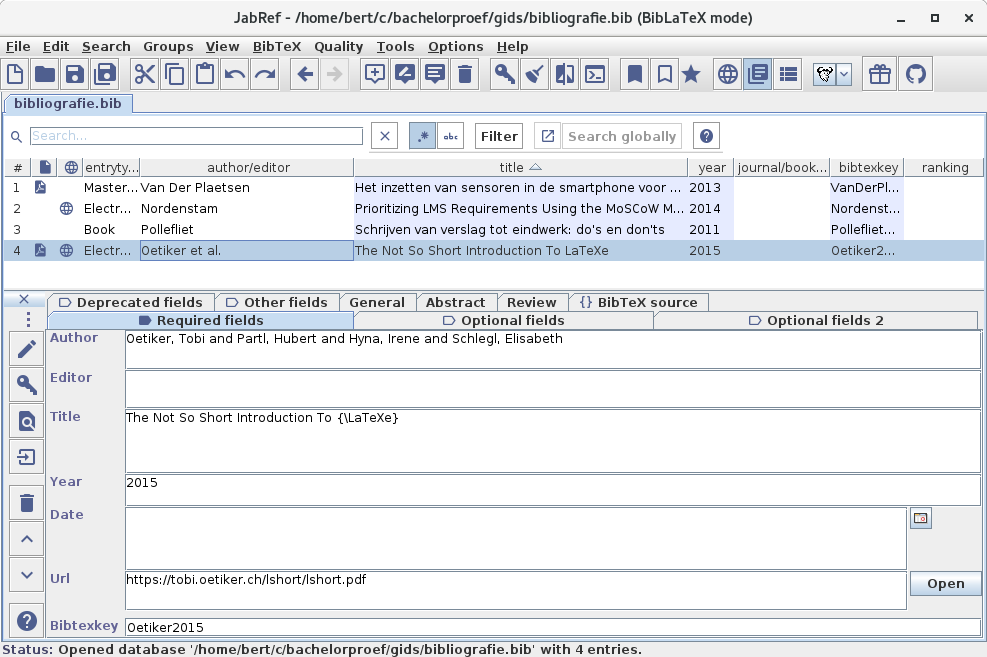
\includegraphics[width=\linewidth]{jabref-screenshot}
  \caption[JabRef]{\textbf{JabRef.} In the center of the user interface you will find an \emph{overview} of the different sources in this bibliographic database, in this case four. The \emph{pdf-icons} on the left of the first and fourth source indicate that the source is stored locally as a PDF. Clicking this will open the PDF. The \emph{globe icons} at the second and fourth source indicate a url that you can open in the web browser when you click on it. At the bottom is a \emph{detail pane} with the tracked data for the fourth source. These are divided into different tabs, including required data (``Required fields''), optional (``Optional'') and others (``Other fields''), etc. In this case, the names of the authors are filled in (see Section~\ref{sub:general_bibliographical_data}). In this case there are no editors (``Editors''), and that field is left empty. The field ``Bibtexkey'' at the bottom is automatically generated (see Section~\ref{sub:jabref_settings}) by clicking on the \emph{key symbol} in the toolbar on the left.} 
  \label{fig:jabref}
\end{figure}

\subsection{JabRef settings}
\label{sub:jabrefsettings}

You can download JabRef from \url{http://www.jabref.org/} and install it on Windows, MacOS and Linux. When you first open JabRef, it is useful to adjust the following settings:

\begin{itemize}
   \item In the menu, choose File > Switch to BibLaTeX mode. This makes the file format of the bibliographic database compatible with the {\LaTeX} template for the bachelor's thesis provided. To adjust this setting, you need to open a bib file.
   \item In the menu, choose Options > Preferences and then the category ``BibTeX key generator''. Each source in the database is identified by a unique key that you can have automatically generated. You can set its shape yourself. The default format is the first author's last name followed by the year of publication, eg ``Knuth1998''. You can adjust this to your own liking, but choose this beforehand and stick to it. You will use this key to refer to your sources from the text, eg with the command \verb|\parencite{Knuth1998}|.
   \item In the Preferences window, choose the File category and specify a directory for keeping PDFs of the sources found under ``Main file directory''. It is very interesting to download the articles found and keep them under that directory. Even better is to take the BibTeX key as the name of the file (eg Knuth1998.pdf). You can then easily open the file from JabRef.   
\end{itemize}

You can check the other settings and adjust them to your liking, but the ones listed above are the most important.

\subsection{General bibliographic data}
\label{sub:general_bibliographic_data}

The purpose of a bibliography is to allow the reader to look up your sources themselves and to assess them for reliability. This means that you must provide sufficient information so that the source can be found. Depending on the type of source (article in a journal, book, website, etc.) you have to provide different information. This will be explored further on. Three elements are \emph{always} essential: the \textbf{author}, the \textbf{title} of the source and the \textbf{year} (or date) of publication. If one of these three is missing, it becomes very difficult to evaluate the origin and quality of the resource. You can keep that kind of sources for information, but they are usually not suitable for inclusion in a bibliography. After all, if the author is unknown, it is not possible to judge whether he or she has the authority to write about the subject in an objective and in-depth manner. If the year is not specified, it is very difficult to determine to what extent this source has not yet been superseded by more recent developments in the field.

Some tips when entering author names:

\begin{itemize}
    
    \item Write the authors' names in the form ``Family Name, First Name(s)''. So ``Van Vreckem, Bert'' and not ``Bert Van Vreckem.'' In principle the second notation is also accepted, but this only works for typical Anglo-Saxon names with a middle name (eg ``Donald Ervin Knuth'' ). The first two words are considered as first names, the last word as the family name. In that case ``Van'' is therefore wrongly regarded as a middle name.
    \item If the author is a company or organization, with a name consisting of several words, enclose it in braces: eg ``\{The Linux Foundation\}''. If not, {\LaTeX} tries to interpret this as a person's name. ``Foundation'' then becomes the family name, ``The'' and ``Linux'' the two first names.
    \item If you have multiple authors, separate each name with \texttt{and}, eg ``Bernard, Anita and Buysse, Jens and Van Vreckem, Bert''.
    \item After entering the author name(s), click on the button with the key icon (see Figure~\ref{fig:jabref}) to generate a unique key for this resource.
    \item In addition to an author field, there is also a field for any editor(s) (\emph{editor}). At least one of the two must be completed, sometimes both. This happens, for example, in a book that is composed of chapters that are written by different authors and where you want to refer to one specific chapter. You will find an example of this further on in this text.   
\end{itemize}

Note that in a bibliography \textbf{only works referenced from the text} may be included. {\LaTeX} does this automatically by default, so if you're missing sources in the list, it means you didn't use them in the text.

Always try to keep as much information as possible about your sources, so that it will be easier to find them later. Although this is a time consuming process, and not all of this information is included in the bibliography, consulting the database is much easier. Pay sufficient attention to this and also check the result in the bibliography itself. Are the authors represented correctly? Do you have a year? Has a URL and date of consultation been specified for an online source (see below)? etc.

Some fields that are always useful to fill in:

\begin{description}
   \item[Abstract] Summary of the article. This is usually the first paragraph of an article and is always clearly marked.
   \item[DOI] or ``Digital Object Identifier''. This is a unique code for articles in scientific publications that makes searching easier (provided the DOI is given).
   \item[File] Name of the file containing the downloaded article. You can open the article from JabRef in a PDF viewer or text editor.
   \item[Keywords] Keywords representing the subject, separated by commas.
   \item[Review] Your own comments about this resource. Why did you keep this? What is the most interesting thing you learned from it?
   \item[URL] The URL where you found the article. This URL is not always included in the bibliography, but it is always useful to keep track of. You can open the website from JabRef in a web browser.
   \item[Urldate] the date on which you last consulted this source.   
\end{description}

\subsection{Specific bibliographic data}
\label{sub:specific_bibliographic_data}

For the most relevant types of sources, this section explains how to properly track and include them in the bibliography. JabRef already gives some indications about which information is at least required: in the details window (see Image~\ref{fig:jabref}) you must at least fill in the tab ``Required fields''. For each type of publication (see Section~\ref{sub:publication types}) below you will find an overview of the fields to be filled in, what they mean exactly, and what the reference in the bibliography will look like.

When adding a new source to a bibliographic database, you must first select the type (see Image~\ref{fig:jabref-entrytypes}). Below we only discuss the most important ones that are relevant for a bachelor's thesis.

\begin{figure}
  \centering
  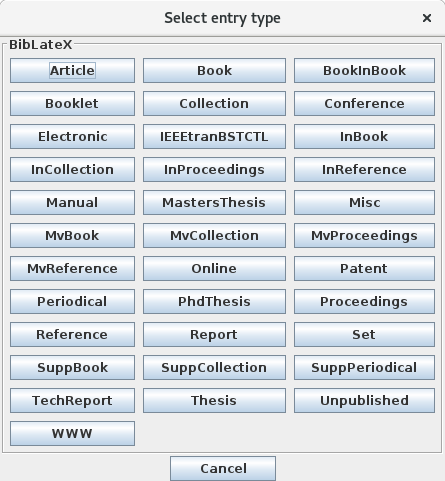
\includegraphics[width=0.6\linewidth]{img/jabref-entrytypes}
  \caption[Types of resources in JabRef]{\textbf{Types of resources in JabRef.} When adding a new resource in JabRef (Ctrl+N) you must first choose the type of publication. Depending on the type, different information must be provided in the bibliography.} 
  \label{fig:jabref-entrytypes}
\end{figure}

\paragraph{Article}

This kind of source is only used for articles published in a scientific journal. Articles in magazines or newspapers are \emph{not} included. Required fields:

\begin{description}
\item[Author] The name of the author;
\item[Title] The title of the article;
\item[Year] Year of publication;
\item[Volume] The volume of the journal in which the article was published;
\item[Number] The number (within the volume) in which the article appeared (sometimes not available);
\item[Pages] Page numbers
\end{description}

Example:
\begin{verbatim}
@Article{SabiEtAl2016,
  author       = {Sabi, Humphrey M. and Uzoka, Faith-Michael E. and
                  Langmia, Kehbuma and Njeh, Felix M.},
  title        = {Conceptualizing a model for adoption of cloud
                  computing in education},
  journaltitle = {International Journal of Information Management},
  year         = {2016},
  volume       = {36},
  number       = {2},
  pages        = {183--191},
  doi          = {10.1016/j.ijinfomgt.2015.11.010},
  url          = {http://www.sciencedirect.com/[...]8401215001115},
  abstract     = {Cloud computing is a pervasive computing [...]},
  keywords     = {Cloud computing, Educational technologies, [...]},
  owner        = {bert},
  timestamp    = {2016-09-01},
}
\end{verbatim}

In the bibliography it looks like this: \fullcitebib{SabiEtAl2016}

\paragraph{InProceedings}

This kind of resource is used for articles published in the proceedings of a \emph{scientific} conference. Required fields:

\begin{description}
 \item[Author] Name of the author(s),
 \item[Title] Title of the article,
 \item[Booktitle] The name of the conference,
 \item[Year] The year in which the conference was held.
\end{description}

You can also optionally fill in the following fields:

\begin{description}
 \item[URL] to the conference website where the article can be found (possibly directly to the PDF);
 \item[Urldate] date on which you last consulted this source.
 \item[DOI] provided one is assigned to this item.
\end{description}

Example:
\begin{verbatim}
@InProceedings{VanVreckemEtAl2013,
  author    = {Van Vreckem, Bert and Borodin, Dmitriy and De Bruyn,
               Wim and Now\'{e}, Ann},
  title     = {A Reinforcement Learning Approach to Solving Hybrid
               Flexible Flowline Scheduling Problems},
  booktitle = {Multidisciplinary International Scheduling Conference
               (MISTA) 2013},
  year      = {2013},
  url       = {https://expertise.hogent.be/files/10711623/hffsp_la.pdf},
  urldate   = {2016-09-01},
  abstract  = {In this paper, we present a method based on Learning
               Automata to solve Hybrid Flexible Flowline Scheduling 
               Problems [...].},
  owner     = {bert},
  timestamp = {2016-09-01},
}
\end{verbatim}

In the bibliography it looks like this: \fullcitebib{VanVreckemEtAl2013}

\paragraph{InBook}

You use this type when you want to refer to a specific chapter in a book. At least the following fields must be completed:

\begin{description}
 \item[Author] The author(s) of the chapter,
 \item[Editor] The editor(s) of the book (if applicable),
 \item[Year] Year in which the book was published,
 \item[Title] Title of the \emph{chapter},
 \item[Pages] Start and end page of the chapter,
 \item[Booktitle] Title of the \emph{book},
 \item[Publisher] Name of the publisher.
\end{description}

Optionally, you can also add the following information:

\begin{description}
  \item[Subtitle or Booksubtitle] subtitle of the chapter or book, respectively,
  \item[Edition] Issue number,
  \item[Location] City where the publisher is located,
  \item[ISBN] The ISBN number of the book (for your information, never shown in the bibliography).
\end{description}

With a book it is unusual to provide a URL. If you want to keep track of the URL of the book on the publisher's website for your own information, it is best to do this in another field, e.g. Comment or Review.

Example
\begin{verbatim}
@InBook{Meyr2008,
  author       = {Meyr, Herbert},
  title        = {Forecast Methods},
  booktitle    = {Supply Chain Management and Advanced Planning},
  year         = {2008},
  editor       = {Stadtler, Hartmut and Kilger, Christoph},
  booksubtitle = {Concepts, Models, Software, and Case Studies},
  edition      = {4e editie},
  publisher    = {Springer},
  location     = {Heidelberg},
  isbn         = {978-3-540-24814-9},
  pages        = {461--472},
  comment      = {https://www.springer.com/us/book/9783540248149},
  owner        = {bert},
  timestamp    = {2016-09-02},
}
\end{verbatim}


In the bibliography it looks like this: \fullcitebib{Meyr2008}

%% TODO: boek, thesis, manual, \ldots

\paragraph{Electronic or Online}

This type of publication includes almost all online sources that cannot be classified under any other category: blog articles, articles in online professional journals or portal sites, YouTube videos of presentations at trade conferences, online documentation, etc.

Note that you may \emph{not} include the general website of organizations, software packages, etc. in your reference list. You can put this in a footnote.

The following fields are required:

\begin{description}
    \item[Author] Author(s) of the source, speaker (in case of a video of a lecture at a conference), \ldots
    \item[Title] Title of source, lecture, \ldots
    \item[Year] Year of publication (or possibly \textbf{Date}, the day of publication, if known),
    \item[URL] to the website where the source can be found,
    \item[Urldate] Date of last consult,
\end{description}

Many errors are made when referencing these types of sources. It is essential that the URL is provided and also the consultation date. The web is constantly changing, and it is possible that the content of a web page changes over time (e.g. bugs that are corrected) or even that a website restructures and thus the URL is no longer valid in some way. By specifying the date of consultation, you still offer the reader the opportunity to find out what that website looked like at that moment in time, for example via the Wayback Machine of the Internet Archive\footnote{\url{https://archive.org/web/}}.

Example of a blog article:

\begin{verbatim}
@Electronic{LewisFowler2014,
  author    = {Lewis, James and Fowler, Martin},
  title     = {Microservices: a definition of this new architectural
               term},
  date      = {2014-03-25},
  url       = {http://martinfowler.com/articles/microservices.html},
  urldate   = {2016-09-01},
  abstract  = {The term "Microservice Architecture" has [...]},
  keywords  = {application architecture, web services, microservices},
  owner     = {bert},
  timestamp = {2016-09-01},
}
\end{verbatim}

In the bibliography this becomes: \fullcitebib{LewisFowler2014}

Another example is one from a presentation at a trade conference that was published on Youtube. Because there is no separate field for mentioning the conference name, it has been incorporated in the title field.

\begin{verbatim}
@Online{Hykes2013,
  author       = {Solomon Hykes},
  title        = {The future of Linux Containers (PyCon 2013)},
  date         = {2013-03-21},
  url          = {https://www.youtube.com/watch?v=wW9CAH9nSLs},
  urldate      = {2016-09-01},
  abstract     = {At PyCon Solomon Hykes shows docker to the
                  public for the first time.},
  owner        = {bert},
  timestamp    = {2016-09-01},
}
\end{verbatim}

In the bibliography: \fullcitebib{Hykes2013}

\section{Searching for relevant information}
\label{sec:Searching_for_relevant_information}

The HOGENT library provides access to a large amount of scientific and professional literature that is not publicly available. This goes far beyond the books available in the library. After all, electronic sources (ebooks, magazines, etc.) can also be consulted. You can also find (good) bachelor's theses from previous years this way. The catalog can be consulted via \url{https://www.hogent.be/student/libraries/}.

\begin{itemize}
  \item Elsevier ScienceDirect
  \item Springer Online Journals
  \item Web of Science
  \item Google Scholar
\end{itemize}

Google Scholar is a search engine for scientific literature that searches both publicly available(``open access'') and paid publications. If you use Scholar from campus or via the VPN, you automatically have access to the publications to which the HOGENT library has a subscription.

Other publicly available search starting points:

\begin{itemize}
 \item Arxiv.org is a database of Open Access articles in a wide range of research domains, including the Computing Research Repository\footnote{\url{http://arxiv.org/corr/home}}.
 
 \item Wikipedia is a good starting point for your research, but remember that Wikipedia articles cannot serve as references themselves. So read the original sources of the article and use them if they are relevant to your bachelor's thesis.
 
 \item There are several portal sites for current ICT-related topics on which technical articles, presentations, interviews, etc. appear, e.g. dzone.com\footnote{\url{https://dzone.com/}}, infoq.com \footnote{\url{https://www.infoq.com/}}, etc.
 
 \item Search for conferences, workshops, symposia, etc. relevant to your field. You don't have to limit yourself to conferences in your own country! Examples are Devoxx\footnote{\url{https://devoxx.be/}} (Java), Google IO\footnote{\url{https://events.google.com/io2016/}} (Android), WWDC \footnote{\url{https://developer.apple.com/wwdc/}} (iOS), Configuration Management Camp\footnote{\url{http://cfgmgmtcamp.eu/}} (Linux Administrative Tools), etc. Lanyrd\footnote{\url{http://lanyrd.com/topics/}} was a website where you could find many conferences on all kinds of topics spread all over the world, but it has been bought by Eventbrite.
 
 More and more conference lectures are filmed and published on Youtube or Vimeo \footnote{For Devoxx for example on \url{https://www.youtube.com/channel/UCCBVCTuk6uJrN3iFV\_3vurg}}. You can also look up the speakers and see if they have published their slides on Slideshare\footnote{\url{https://slideshare.net/}} or Speakerdeck\footnote{\url{https://speakerdeck.com/}} .
 
   \item Are there any local associations that are interested in your field? For example OWASP Belgium\footnote{\url{https://www.owasp.org/index.php/Belgium}} (security of mobile and web applications). You can search for such groups via Meetup\footnote{\url{https://meetup.com/}} or also via LinkedIn\footnote{\url{https://www.linkedin.com/}} (search specifically for groups such as the Belgian IT Infrastructure Network\footnote{\url{https://www.linkedin.com/groups/2092569}}). Check if there are any upcoming events near you and go there.
  
  \item Who are the most important names in the ``community''? Keynote speakers at conferences, authors of the most important books on the subject, etc. Follow these people on Twitter, find out if they have a blog, are active on LinkedIn, etc. Read all you can find they've written in the latest years.
  
  \item Find out if there are newsletters about your subject, which periodically send updates about current events in that field. Examples are Cron.Weekly\footnote{\url{https://www.cronweekly.com/}} (Linux System Administration), DevOps Weekly\footnote{\url{http://www.devopsweekly.com/}} or JS Weekly (and relatives)\footnote{\url{https://javascriptweekly.com/}}.
\end{itemize}

Keeping track of all your sources is time-consuming, but essential for a sound bachelor thesis! So pay the necessary attention to this and check whether the information about your sources is entered correctly in JabRef.

All relevant information that you have collected and read in the course of your research is then synthesized in a continuous text in your own words where you discuss the situation in the research domain, with references to the literature at appropriate places. We will go into more detail in Chapter~\ref{ch:writing}.

\section{Summary}
\label{sec:bibliography-summary}

\begin{itemize}
    \item Set up your bibliographic database (e.g. with JabRef) before looking for information on your subject and store as much information as possible.
    \item Make sure you always write down at least the author, title and year of publication. Check for all other information required for this type of publication.
    \item In addition to consulting accessible sources, it is also interesting to find information about your subject via the HOGENT library.
    \item Use the APA style. 
\end{itemize}

\chapter{Research methods}
\label{ch:researchmethods}

In this chapter you will find recommendations related to some commonly used research methods. More specifically, we discuss the approach of a comparative study, how to correctly set up experiments and how to report correctly on the results obtained (in particular figures).

% Belang van correcte methodologie
%
% Voorbeelden:
% - enquêtes (verwijzen naar Saunders?)
%     - pitfalls: respons, slechte vragen, slechte verwerking, te laat opgengesteld
%     - onderzoekskader, steekproefmethode (benader aselecte steekproef)
%     - stel vragen zo dat je op zoek kan gaan naar verbanden!
%     - tip: neem deel aan enquêtes, bv. van iMinds => voeling met vraagstelling
% - interviews (kwalitatief)
%     - wanneer? Casus leren kennen, vakexpert, requirements-analyse
%     - Goed voorbereiden, opnemen, transcriptie uitschrijven, verwerken
% - experiment
% - vergelijkende studie
% - casus/case study
% - doorlichting beveiliging: risico-analyse Chris Jackson, Network Security Auditing. Cisco Press. 2010.
%
% wanneer pas je elk toe?
% Vaak heb je een combinatie van deze technieken nodig om je onderzoeksvra(a)g(en) goed en onderbouwd te kunnen beantwoorden.

\section{The comparative study}
\label{sec:comparativestudy}

A topic that is often chosen for a bachelor's thesis is a comparative study. You are looking for a solution for a problem in the form of a software or hardware product, platform, service, etc. The aim of the study is to compare all possible alternatives and to make a choice for the most suitable one.

Experience shows that a comparative study is only really good if there is a concrete goal, a real situation where the selected solution will actually be applied. There is a threat that the study will be limited to listing a few arbitrarily chosen options. A section of explanation follows, sometimes simply taken from Wikipedia, with a summary of some advantages and disadvantages, but not structured and without a common thread. A certain aspect such as ``user-friendliness'' is then discussed in one product, but not for the other, etc. Your own input is then minimal: a day's search on Wikipedia, summarize or further write it out, done. This is therefore insufficient.

But how \emph{do} you go about then?

Let's assume that you want to work as a web developer after graduation, and you are looking for a suitable PHP framework to build your websites with.

\subsection{Requirements-analysis}
\label{ssec:requirements-analysis}

To make a good choice, start by collecting \emph{requirements}, both \textit{functional} and \emph{non-functional}, e.g.:

\begin{itemize}
\item Functional requirements
  \begin{itemize}
 \item HTML5/CSS3 support
 \item Responsive design
 \item It must contain an authentication module that supports OpenID, Facebook and Google authentication
  \item \ldots
  \end{itemize}
\item Non-functional requirements
  \begin{itemize}
 \item Must be able to withstand OWASP's top-10 vulnerabilities\footnote{\url{https://www.owasp.org/index.php/Category:OWASP_Top_Ten_Project}}
 \item Passwords are stored according to the state-of-the-art (\emph{salted} and \emph{hashed})
 \item Must be open source
 \item Must be free
  \item \ldots
  \end{itemize}
\end{itemize}

If you are doing the research for a ``client'' (i.e. your co-promoter), then you naturally involve all stakeholders in this process! You list the requirements and divide them according to importance, for example using the MoSCoW technique~\parencite{Nordenstam2014}. You then divide the requirements into categories such as ``must-have'', ``should-have'' and ``nice-to-have''.

\subsection{Long list}
\label{ssec:long-list}

Then you look for \emph{as many as possible} alternatives that are eligible to be used, i.e. ~all the ones you can find. You mention them in this \emph{long list} (which can sometimes consist of dozens of alternatives) by name, possibly mentioning a website and a description in one sentence. You check each alternative against the requirements, if this is possible already based on the information that you find on the website or from other sources. You just leave things you can't verify to check later or maybe even ignore them (e.g. if it's an insignificant feature, or if several other must-haves aren't met). You then sort the long list according to the number of requirements met, and make a clear table of this. Hopefully you've been left with some alternatives that meet all the must-haves and as many should-haves and nice-to-haves as possible.

\subsection{Short list and proof-of-concept (POC)}
\label{ssec:short-list-poc}

Keep the most promising alternatives for the next phase. You will discuss the alternatives in this \emph{short list} in more detail and compare them further. If necessary, set up a \emph{proof-of-concept} (see Section \ref{sec:poctestsetup}), in which you try out one or more of the most promising alternatives based on the same defined \emph{scenario} in which you discuss the requirements that you have not yet been able to verify.

\subsection{Conclusion}
\label{ssec:comparativestudyconclusion}

Finally, you give your \emph{recommendation}, the alternative that best meets the requirements, and what else needs to be done to make it even more suitable.

\section{Proof-of-concept or test setup}
\label{sec:poctestsetup}

With a proof-of-concept or test setup you want to demonstrate that a proposed or promising solution for the research question can also be realized in practice. It is often necessary to set up different variants next to each other, so that you can still compare.

A good test setup satisfies three properties \autocite{Liberman2015}:

\begin{description}
  \item[Reproducibility] be able to rebuild the test setup (possibly by an independent party) and run the analysis again so that you can verify that you get similar results.
  \item[Replicability] is similar to the above, but expressed more strongly: with a replicable test set-up it is possible that an independent party can repeat this \textit{exact} setup and obtain the same results.
  \item[Reusability] can set up variants of the test environment so that they can be compared.
\end{description}

The best way to achieve this is to automate the process.

\subsection{Reproducibility}
\label{ssec:reproducibility}

A minimum expectation of a bachelor's thesis text is that the reader must be able to reproduce the test set-up on the basis of the description and must be able to verify your conclusions. That also means that your description must be sufficiently detailed. At the beginning of this section, give a clear picture in your text with a schema of the set up test environment. Then describe in detail:

\begin{itemize}
 \item What hardware was used? Computers, network equipment, other ICT infrastructure. What specifications do these devices have (CPU, memory, hard drive type and size, network interface speed, etc.)?
 \item Which software packages are installed that are relevant for the test setup? Which specific editions and/or version numbers?
 \item How exactly did the installation procedure go? Which settings have been adjusted, and how are all components configured?
\end{itemize}

\subsection{Replicability}
\label{ssec:replicability}

It is important for both you and the reader of your bachelor's thesis to automate the setting up of the test environment as much as possible, for example by writing an installation script. In this way you achieve the \textit{replicability} of your test setup.

For many situations you can develop a proof-of-concept with virtual machines. In this way you create a protected environment without having to install additional software on your physical system. Vagrant\footnote{\url{https://www.vagrantup.com/}} is an interesting tool to set up fully automated reproducible virtual test environments. It is not itself a virtualization system, but it addresses VirtualBox, VMWare or Hyper-V from the command-line. You describe in a configuration file (\texttt{Vagrantfile}) which VMs you need, with how many processor cores/memory/disk space, with which operating system, etc. Via a script or configuration management system (such as Ansible) you can determine the precise configuration of the Describe VMs (software installation, users, network services, configuration files, etc.). The code/configuration to set up a Va\-grant-\ environment is very compact, completely text-based and thus can be maintained in a version control system.

Docker\footnote{\url{https://docker.com/}} is also an interesting tool for this. Docker is a form of so-called container virtualization. Virtual machines (containers) do not have their own OS, but in principle only contain an application. The OS of the physical system is reused by the containers. This makes containers a lot more efficient in terms of disk and memory usage for the physical system. However, there are a number of limitations that make Docker not always useful as a platform for a test setup.

If you notice that you have made a mistake in the configuration of your test setup, you can adjust the installation script and set up the entire test environment again. If you had to do this manually, you might lose at least a day. In addition, there is a chance that you will overlook a small detail and therefore not be able to replicate the test environment exactly again. Initializing a Linux VM with Vagrant or Docker typically only takes a few minutes. Windows systems take a lot more time. The OS itself is a lot bigger\footnote{Approx.~4GB for Windows Server Core compared to 256 to 512MB for a minimal installation of a Linux distribution. Application installations have an additional impact on the disk size of the VM.}

A comprehensive tutorial of Vagrant or Docker is beyond the scope of this guide. An example to illustrate can be found at \url{https://github.com/bertvv/lampstack}. Here an Apache web server is set up with a MariaDB database, PHPMyAdmin, and Wordpress.

\subsection{Reusability}
\label{ssec:reusability}

By automating the entire process, you create an additional advantage: it is a lot easier to create similar variants of a test setup. Suppose you want to measure the performance impact of a cache on a database system. The installation of both variants (with/without cache) are very similar. In a Vagant environment you can create 2 VMs, with the same installation script for the basic setup, and a separate script to realize the different configuration variants.

\section{Conducting experiments and collecting quantitative data}
\label{sec:conductingexpertiments}

When you set up an experiment in which you are going to collect quantitative data, for example for a performance comparison, the same guidelines apply as for a proof-of-concept: it is important that it is reproducible, replicable and reusable. You may start from a predefined test setup, and you will repeatedly perform the same action and take measurements.

Here too it is important to automate the execution of the experiment and to save your test results, for example by means of a shell script. If you have to perform an experiment manually, this quickly becomes a very time-consuming activity. Imagine that every time you want to run the experiment you have to press a button, wait about five to ten minutes and then copy and paste the output to Excel and then edit the spreadsheet again so that you are only left with the numbers to statistically to process. This method is untenable. After all, you have to be constantly present and attentive while performing. Moreover, with every manual operation there is a chance of making mistakes.

A script that can run the experiment in different variants without user interaction, and also immediately saves the results in a suitable file format saves you a lot of time. You can run the experiment overnight and that way you can repeat it enough to get statistically useful results. If an experiment fails, all you need to do is improve the script and run it again. It is also easier to write different variants (like the earlier example of database queries with or without cache).

% TODO:
% - vergelijk je de juiste dingen? Zijn neveneffecten uitgeschakeld?
% - Experimenten vele keren herhalen

% Valkuilen: enquêtes, ...
\chapter{Resultaten rapporteren}
\label{ch:resultaten-rapporteren}

%
% Een scriptie is een afgesloten geheel. Alle informatie die nodig is om het onderwerp ten gronde te begrijpen moet er in zitten. Het mag dus niet nodig zijn om nog externe bronnen na te lezen voordat je de tekst kan begrijpen.
% Dat betekent o.a. dat je specifieke vaktermen binnen het domein moeten verklaard worden!

Op een bepaald moment heb je een heleboel informatie verzameld en geanalyseerd, en wordt het tijd om het finale document op te maken. In dit hoofdstuk vind je enkele tips en richtlijnen om tot een goed resultaat te komen.

In deze gids beperken we ons tot enkele belangrijke punten en specifieke aanbevelingen voor de opmaak van de tekst in {\LaTeX}. Een meer omvattend overzicht kan je o.a.~vinden in het boek van~\textcite{Pollefliet2011}.

\section{Algemene richtlijnen}
\label{ch:algemene-richtlijnen}

Wanneer je een tekst schrijft wil je uiteraard je best doen om deze zo aangenaam mogelijk te maken om te lezen. Er zijn echter een aantal dingen waar je moet op letten. In je bachelorproef toon je aan dat je een professionele instelling hebt en een gezonde dosis maturiteit op zak hebt. Dat moet ook tot uiting komen in je schrijfstijl. De tekst moet professioneel en objectief overkomen. Vermijd in het bijzonder volgende zaken:

\begin{itemize}
  \item Schrijven vanuit je eigen standpunt is uit den boze. Gebruik dus nooit de \textbf{ik-vorm}. Die geeft immers de indruk dat je je \emph{eigen mening} geeft, en als junior in je vakgebied heb je daarvoor onvoldoende autoriteit. De beweringen die je in je bachelorproef doet moeten objectieve aantoonbare feiten zijn, die ofwel gesteund worden door een verwijzing naar gezaghebbende vakliteratuur, hetzij volgen uit je eigen onderzoeksresultaaten.
  \item Gebruik geen \textbf{spreektaal}. Blijf formeel en zakelijk.
  \item Gebruik geen \textbf{vage termen} om een hoeveelheid aan te duiden, bv. lang, groot, snel, populair, \ldots Quantificeer al deze uitspraken met cijfers en meeteenheiden (uiteraard ondersteund door literatuurverwijzingen of resultaten van eigen onderzoek).
  \item Gebruik geen \textbf{toekomstige tijd.} Op het moment dat je afgewerkte bachelorproef gelezen wordt, is het een verslag van in het verleden uitgevoerd onderzoek. Dus niet ``Eerst zal worden gekeken naar\ldots'' maar ``Eerst werd onderzocht\ldots''
\end{itemize}

% http://www.taalwinkel.nl/schrijfproces/een-wetenschappelijke-schrijfstijl/
% familiair (je), ``populariserend''

% Voorbeeld vage termen:
% ``Doorheen de laatste jaren zijn mobiele applicaties enorm ge-
% groeid''
% Bron -> http://blog.appfigures.com/app-stores-growth-accelerates-in-2014/
% Gebruik waar mogelijk Nederlandse termen en vermijd Anglicanismen. Als er een Nederlands woord voor bestaat gebruik je dat, en niet de Engelse term. Bv. tree -> boom, deployen -> uitrollen, enz.

% Een zin = een gedachte
% Een paragraaf = bij elkaar horende gedachten die één onderwerp, redenering vormen
% Tip: De eerste zin van een paragraaf bevat de hoofdgedachte van de paragraaf, de andere zinnen leggen die verder uit, of gaan er dieper op in.
%
% Samengestelde woorden hangen aan elkaar: informatiebeveiliging ipv informatie beveiliging

Hou rekening met je \emph{doelpubliek}. In principe kan je er van uitgaan dat de lezer een ict-achtergrond heeft (tenzij je je onderwerp uitwerkt in samenwerking met of in opdracht van iemand uit een andere discipline). Je kan dus meestal een zekere basiskennis veronderstellen, maar termen en afkortingen die specifiek zijn voor je eigen onderzoeksdomein moet je zeker uitleggen.

Doe een \emph{grondige controle} op spellings- en grammaticale fouten. Deze \emph{moeten} er uit zijn bij indienen. Voor een informaticus telt elke punt en komma. Een tekst vol fouten geeft een heel slechte indruk over je capaciteiten.

Begin elk hoofstuk (en sectie) met een inleidende paragraaf die aangeeft wat de inhoud ervan is wat de link is met het vorige hoofdstuk. Iemand die meteen dat hoofdstuk begint te lezen krijgt op die manier wat context.


% Volgorde van schrijven (samenvatting laatste)

%- Conclusie, samenvatting, voorwoord schrijf je het laatste maar het is vaak het eerste dat gelezen wordt. Bijzonder veel aandacht aan schenken
    %- Conclusie moet terug grijpen op de onderzoeksvraag
    %- Bedenkingen, future work
    %- Samenvatting is geen voorwoord. Moet maw. ook belangrijkste conclusies bevatten

% LaTeX tips
%
% Aanhalingstekens: er bestaan geen smart quotes
% - links: backquote, rechts single quote
% - dubbele aanhalingstekens: `` en ''

% Titel:
% - concreet, niet enkel het onderzoeksdomein benoemen
% - Geef het onderwerp, niet een onderzoeksvraag
% - Gebruik geen afkortingen en vermijd jargon
% - Vermijd algemene, nietszeggende woorden. vb. ``Studie,''  ``Onderzoek naar'' -> een bachelorproef is altijd een onderzoek

% Einde inleiding: Sectie ``Opzet van deze bachelorproef''
% De rest van deze bachelorproef is als volgt opgebouwd:
%
% In hoofdstuk N \ldots
% In hoofdstuk N+1 \ldots
% \ldots

\section{Afbeeldingen}
\label{sec:afbeeldingen}

Het invoegen van afbeeldingen in een {\LaTeX}-document is \'e\'en van de struikelblokken voor beginnende gebruikers van het tekstzetsysteem. In een klassieke WYSIWYG tekstverwerker ben je gewend om zelf te bepalen waar een afbeelding op het papier terecht zal komen. Meestal doe je dat dan meteen onder het deel van de tekst waar naar de afbeelding verwezen wordt. In een groter document wordt dit problematisch. Het is immers mogelijk dat door toevoegingen van tekst vóór de afbeelding, die de ondermarge gaat overschrijden. De tekstverwerker zal dan wellicht de afbeelding naar de volgende bladzijde verplaatsen en je krijgt onderaan extra witruimte. Dit ziet er niet goed uit, en je verliest dan kostbare tijd met het goed positioneren van de afbeeldingen ten opzichte van de tekst.

{\LaTeX} kan zelf bepalen waar een afbeelding het best gepositioneerd wordt. Het is in eerste instantie vervelend om deze controle te moeten afstaan, maar de bladspiegel zal er wel een stuk beter door uitzien. Soms kiest {\LaTeX} er voor om de afbeelding een bladzijde verder of eerder te plaatsen dan de tekst die er op betrekking heeft. Dat betekent dus dat de context voor de afbeelding niet meer bij de afbeelding staat. Dit kan je echter oplossen door bij elke afbeelding een bijschrift (\emph{caption}) te plaatsen dat volledig beschrijft wat er op de afbeelding te zien is. Beperk je niet tot enkele woorden. Gebruik volledige zinnen zodat de lezer de afbeelding kan begrijpen zonder naar de bijhorende tekst te moeten gaan zoeken. In de tekst zelf verwijs je dan uiteraard naar de afbeelding (met \verb|\ref{fig:label}|).

% TODO: template voor invoegen van afbeelding

Onder de auteurswetgeving is het toegelaten om binnen de context van onderwijs afbeeldingen uit andere publicaties over te nemen zonder voorafgaande toestemming van de auteur. Het is dan uiteraard essentieel dat je in het bijschrift een literatuurverwijzing toevoegt. Zoniet wordt dit beschouwd als plagiaat.

Logo's van producten of bedrijven toevoegen is \emph{geen} goed idee. Dit valt immers niet enkel onder de auteurswetgeving, maar onder de merkenwet. Een logo weerspiegelt de identiteit van een bedrijf en het gebruik van het logo wordt dan ook sterk gecontroleerd (grootte, correct kleurgebruik, enz.). Derden mogen enkel na expliciete toestemming en onder specifieke voorwaarden het logo gebruiken. In een thesis voegt een logo trouwens geen enkele inhoudelijke meerwaarde toe, wat op zich al een reden is om er geen in te voegen.

Wanneer je een afbeelding overneemt van een website, zorg er dan zeker voor dat de resolutie voldoende hoog is. Afbeeldingen die er op een beeldscherm goed uitzien, kunnen op papier duidelijk de individuele pixels zichtbaar worden, wat niet goed overkomt. Een beeldscherm heeft typisch een veel lagere resolutie (96 DPI of \emph{dots per inch}, beeldpunten per duim) dan een printer (300 of 600 DPI). Voor een goed resultaat moet een afbeelding minstens evenveel pixels bevatten als de gewenste hoogte of breedte van de afbeelding op papier, vermenigvuldigd met de resolutie. Als je dus bijvoorbeeld een afbeelding op $5 \times 5$ cm (of ongeveer 2 inch) wil afdrukken op een 300 DPI printer, moet je afbeelding minstens $600 \times 600$ pixels groot zijn.

Een alternatief is werken met \emph{vector graphics}, m.a.w.~figuren die in het document getekend worden aan de hand van wiskundig gedefinieerde vormen. Er bestaat een zeer uitgebreide package voor {\LaTeX} hiervoor: Ti$k$Z. Dit heeft wel een steile leercurve, maar het resultaat is wel van hoge kwaliteit. Een inleiding op Ti$k$Z valt buiten de scope van deze gids, maar er zijn veel tutorials en voorbeelden te vinden op het Internet\footnote{Bijvoorbeeld \url{http://www.texample.net/tikz/}}.


% Voldoende hoge resolutie voor screenshots (gekopieerd van webpagina): http://brandonmathis.com/blog/2010/10/08/how-to-get-high-resolution-screenshots-of-a-website
% Kleurenpallet (contrast, toeg
% tikz (maar dat is een specialiteit op zich\ldots)
%
% Index? Woordenlijst?

% TODO: SECTIE: de literatuurstudie schrijven
%
% De literatuurstudie/state-of-the-art is een doorlopende tekst waarin je in je eigen woorden de situatie in het onderzoeksdomein schetst, met op gepaste plaatsen verwijzingen naar de literatuur. Expliciet schrijven ``in het artikel X van Y heb ik Z gelezen'' wordt niet gedaan. Lees een aantal wetenschappelijke publicaties over je onderwerp en probeer die stijl na te volgen.
%
% Wanneer verwijzen naar de literatuur:
% - Elke introductie van domeinspecifieke vaktermen
% - Elke bewering over het vakdomein (die je quantificeert!)
% - Elke verwijzing naar resultaten vorig onderzoek
%
% Twee commando's: (Auteur, jaar) of Auteur (jaar)


\section{Visualisatie van cijfermateriaal}
\label{sec:visualisatie-cijfermateriaal}

In de cursus Data Science \& AI wordt het goed visualiseren van cijfermateriaal in detail besproken en geoefend. Toch zien we dat in de bachelorproef nog heel veel fouten gemaakt worden met foute conclusies als gevolg. Daarom komen we hier nog even terug op dit onderwerp.

% - Enkel gemiddeldes vermelden is onvoldoende! Minstens ook standaardafwijkingen geven en statistische toetsen uitvoeren om te verifiëren of resultaten significant verschillen.

Stel, je voert een performantievergelijking uit tussen twee systemen, A en B. Je hebt op elk systeem 50 keer een experiment uitgevoerd en de resultaten geregistreerd. Laat ons veronderstellen dat het resultaat van de meting een 

\begin{figure}
  \begin{subfigure}{.5\textwidth}
    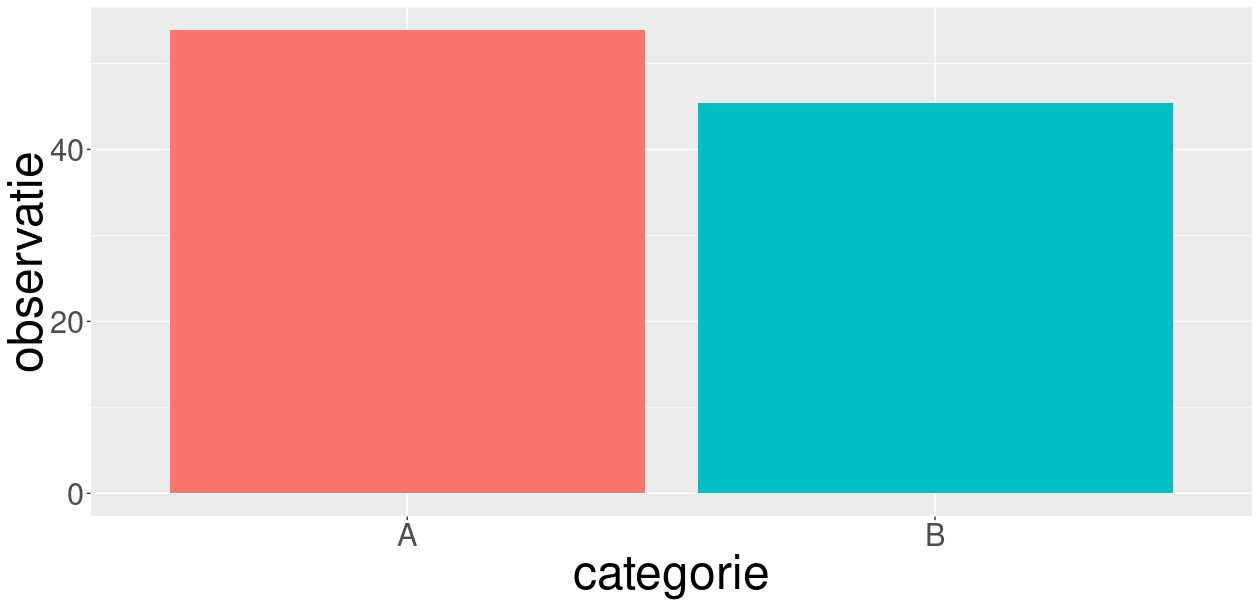
\includegraphics[width=\textwidth]{voorbeelden/barplot.png}
    \caption{Staafdiagram van gemiddelden. Dit is onvoldoende om een conclusie te trekken}
    \label{fig:barplot}
  \end{subfigure}
  \begin{subfigure}{.5\textwidth}
    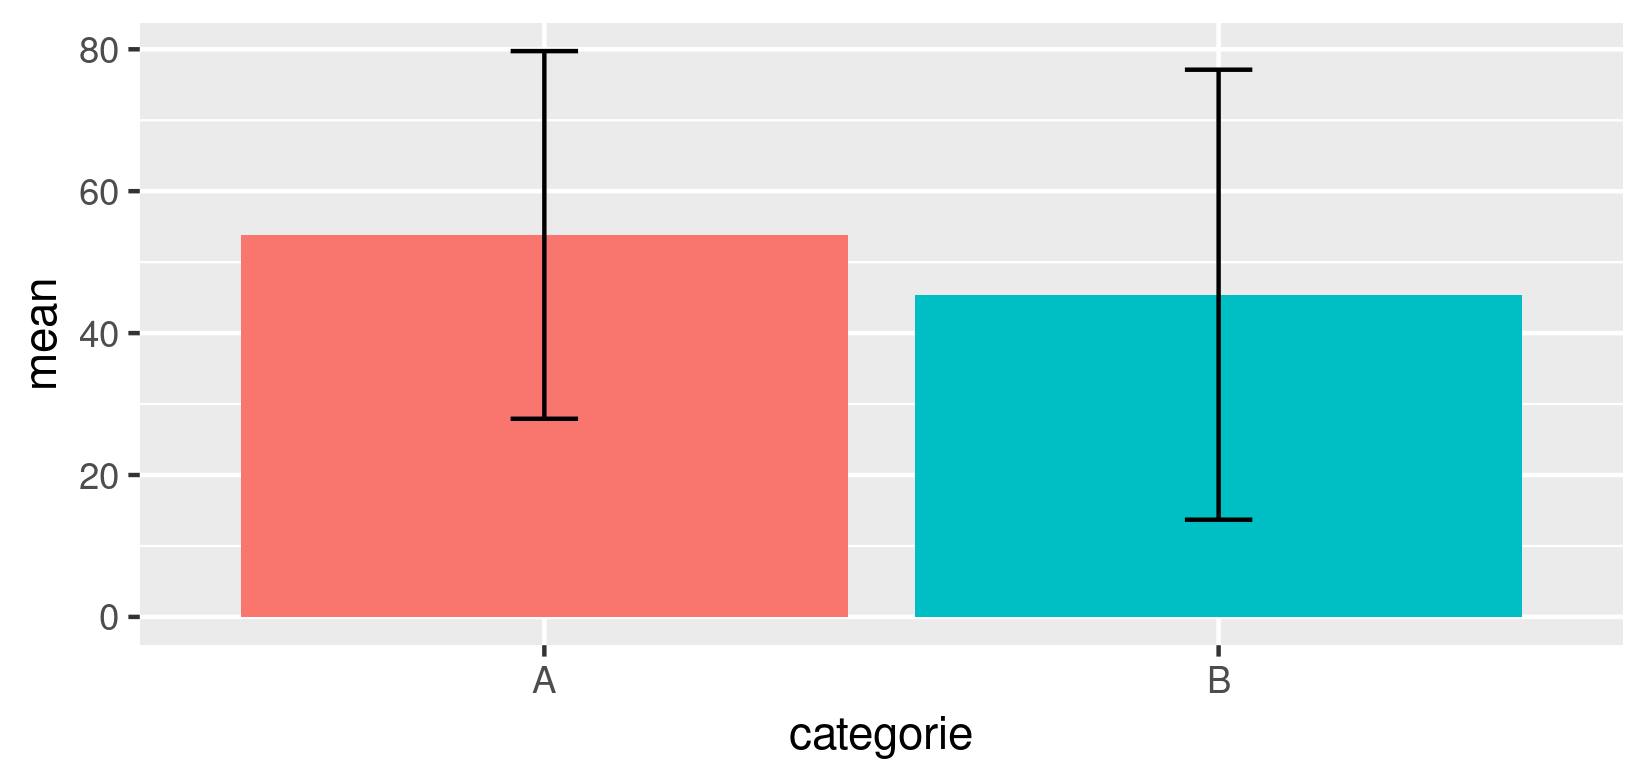
\includegraphics[width=\textwidth]{voorbeelden/barplot-errorbars.png}
    \caption{Staafdiagram met \textit{error bars} die de grootte van de steekproefstandaardafwijking voorstellen. Door de grote spreiding is het verschil tussen beide categorieën ineens veel minder uitgesproken.}
    \label{fig:barplot-errorbars}
  \end{subfigure}
  
  \begin{subfigure}{.5\textwidth}
    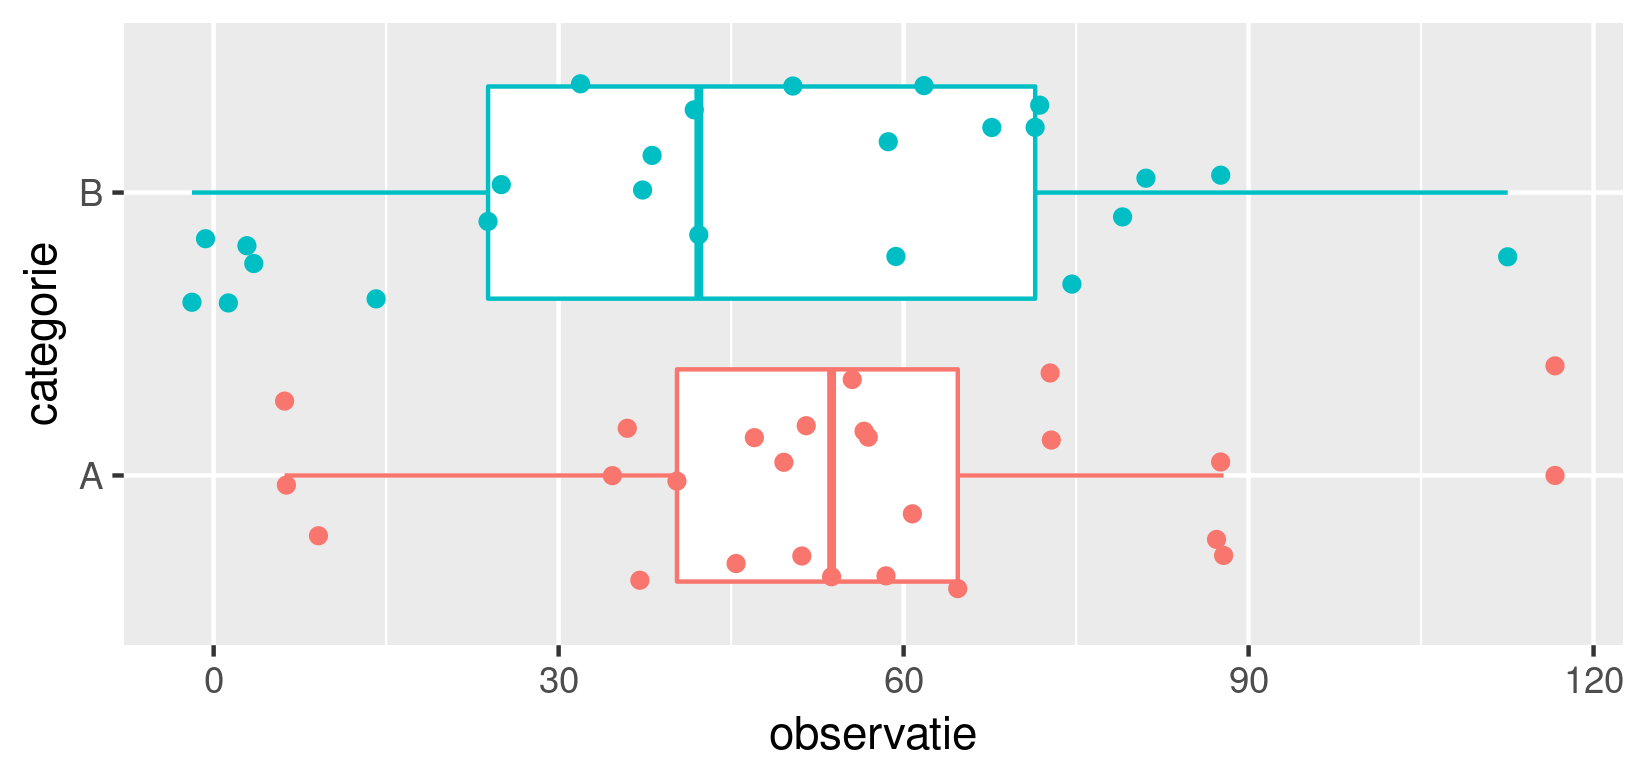
\includegraphics[width=\textwidth]{voorbeelden/boxplot-jitter.png}
    \caption{Boxplot met individuele observaties weergegeven als punten. Hiermee is de spreiding van de data nog duidelijker.}
    \label{fig:boxplot-jitter}
  \end{subfigure}
  \begin{subfigure}{.5\textwidth}
    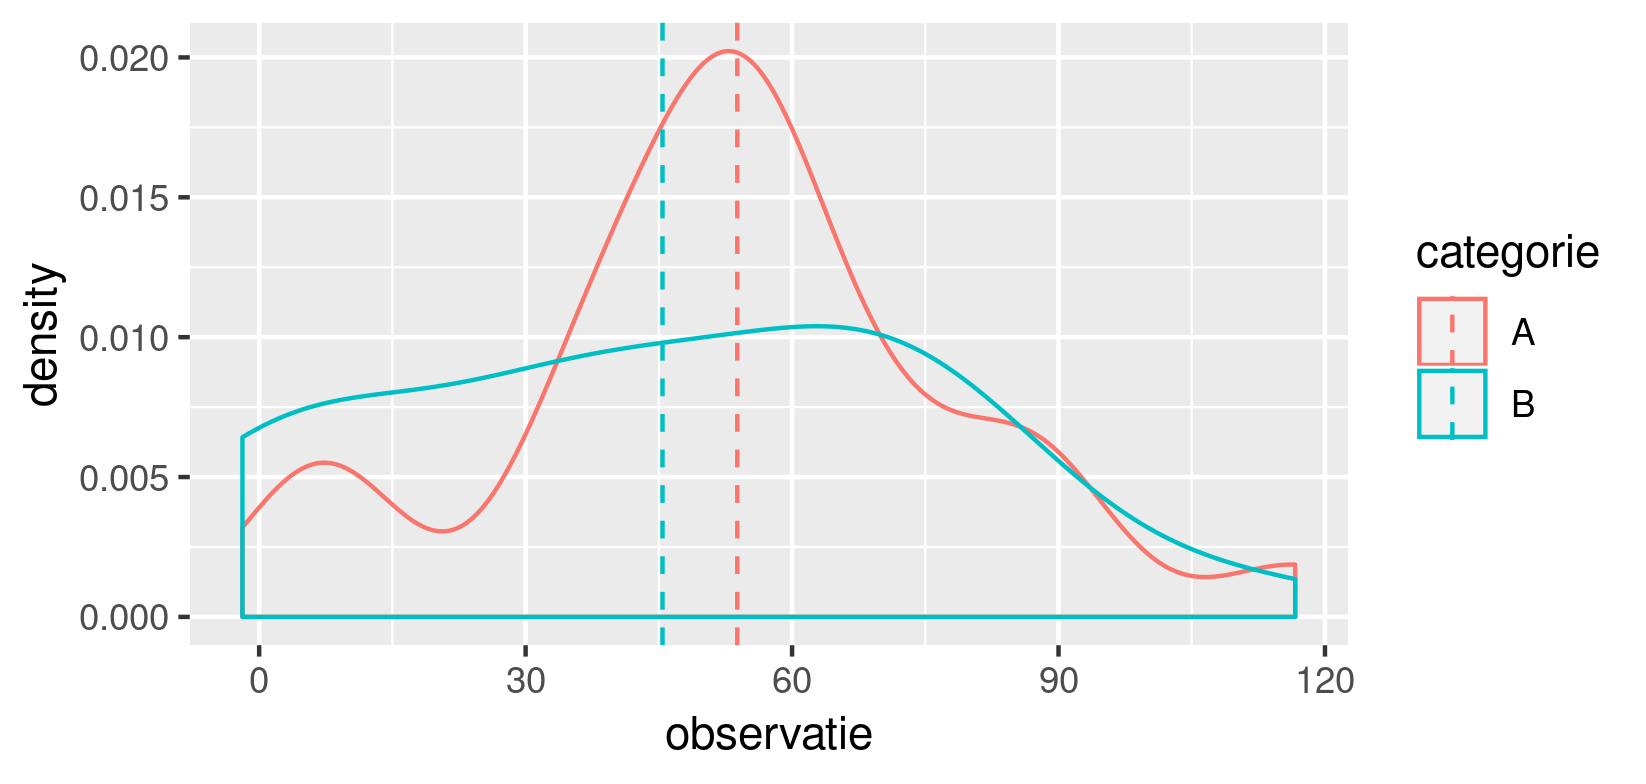
\includegraphics[width=\textwidth]{voorbeelden/density-plot.png}
    \caption{Kansdichtheid met steekproefgemiddelden aangeduid als een verticale stippellijn. Hier wordt duidelijk dat de resultaten van het experiment niet normaal verdeeld zijn. Dat maakt dat een staafdiagram met error bars eigenlijk niet geschikt is voor deze data.}
    \label{fig:density-plot}
  \end{subfigure}
  
  \caption[Visualiseren van cijfergegevens]{Verschillende manieren om dezelfde data te visualiseren.}
\end{figure}



%---------- Back matter -------------------------------------------------------
% In de bibliografie niet de bronnen uit voorbeeld.bib afdrukken. Alle bronnen
% in voorbeeld.bib moeten in het veld ``keywords'' ook de term ``voorbeeld''
% bevatten.
\printbibliography[notkeyword=voorbeeld]
\addcontentsline{toc}{chapter}{\textcolor{title}{\IfLanguageName{dutch}{Bibliografie}{Bibliography}}}

\end{document}
